% ★★ 中档
\newcommand{\qConicDefZeroAngleStem}{
如图，斜线段 $AB$ 与平面 $\alpha$ 所成的角为 $\frac{\pi}{4}$，$B$ 为斜足．平面 $\alpha$ 上的动点 $P$ 满足 $\angle PAB = \frac{\pi}{6}$，则点 $P$ 的轨迹为（\quad）
}
\newcommand{\qConicDefZeroAngleOptions}{
\mcoptions[4]{圆}{椭圆}{双曲线的一部分}{抛物线的一部分}
}
\newcommand{\qConicDefZeroAngleFigure}{
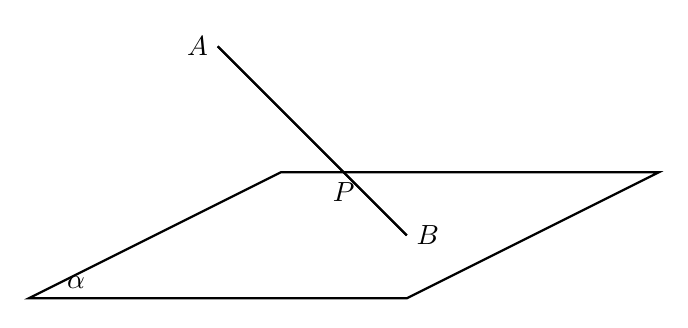
\begin{tikzpicture}[scale=0.8, x={(1cm,0cm)}, y={(0.5cm,0.5cm)}, z={(0cm,1cm)}]
  % Plane alpha
  \draw[thick] (-2,-2,0) -- (4,-2,0) -- (6,2,0) -- (0,2,0) -- cycle;
  \node at (-1.5,-1.5,0) {$\alpha$};
  % Point B
  \coordinate (B) at (3,0,0);
  \node[right] at (B) {$B$};
  % Point A
  \coordinate (A) at (0,0,3);
  \node[left] at (A) {$A$};
  \draw[thick] (A) -- (B);
  % Point P
  \coordinate (P) at (1,2,0);
  \node[below] at (P) {$P$};
  \draw[thick] (A) -- (P);
  \draw[thick] (B) -- (P);
\end{tikzpicture}
}
\newcommand{\qConicDefZeroAngleAnswer}{
B
}
\newcommand{\qConicDefZeroAngleSolution}{
根据圆锥截面定义（第零定义），将直线 $AB$ 视作圆锥的旋转轴，平面 $\alpha$ 视作截面。\\
由题意，圆锥的母线（如直线 $AP$）与旋转轴 $AB$ 的夹角（半顶角）为 $\theta = \frac{\pi}{6}$。\\
平面 $\alpha$ 与旋转轴 $AB$ 所成的线面角为 $\beta = \frac{\pi}{4}$。\\
比较可知，$\theta = \frac{\pi}{6} < \beta = \frac{\pi}{4} < \frac{\pi}{2}$。\\
当线面角 $\beta$ 大于母线与轴的夹角 $\theta$ 时，截面与圆锥的所有母线都相交，故截得的曲线是椭圆。
}
\newcommand{\qConicDefZeroAngleDiagnosis}{
\errortag{线面角混淆} 学生容易把平面与轴线的线面角 $\beta$ 误认为是平面与底面的二面角。\\
\errortag{母线角混淆} 学生可能没有意识到 $\angle PAB$ 就是旋转面（圆锥）的母线角。
}
